% !TEX TS-program = xelatex
% !TEX encoding = UTF-8 Unicode
% !Mode:: "TeX:UTF-8"

\documentclass{resume}
\usepackage{graphicx}
\usepackage{tabu}
\usepackage{tabularx}
\usepackage{multirow}
\usepackage{progressbar}
\usepackage{zh_CN-Adobefonts_external} % Simplified Chinese Support using external fonts (./fonts/zh_CN-Adobe/)
\usepackage{tikz}
% \usepackage{NotoSansSC_external}
% \usepackage{NotoSerifCJKsc_external}
% \usepackage{zh_CN-Adobefonts_internal} % Simplified Chinese Support using system fonts
\usepackage{linespacing_fix} % disable extra space before next section
\usepackage{cite}

\newcommand{\hlink}[1]{\href{#1}{#1}}

\begin{document}
\pagenumbering{gobble} % suppress displaying page number

\medskip\noindent
\begin{minipage}{0.7\textwidth}
  \large{
    \begin{tabu}  { l }

      \Huge{\scshape{覃\ 缘}} \\
\ \\
      \email{xiaojkql@163.com} \\
      \phone{(+86) 132-0179-8186} 
	%期望岗位:{NLP算法工程师}
    \end{tabu}
  }
\end{minipage}
\begin{minipage}{0.3\textwidth}
  \raggedleft
  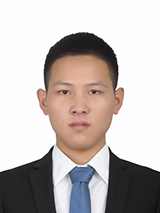
\includegraphics[height=30mm]{me}
\end{minipage}

% \name{唐宗勋}
%
% \basicInfo{
%   \email{tangzongxun@hotmail.com} \textperiodcentered\ 
%   \phone{(+86) 13070156080} \textperiodcentered\ 
%   \linkedin[tangzongxun]{https://www.linkedin.com/in/tangzongxun}}


\section{教育背景}
\datedsubsection{\textbf{西安交通大学}, 西安}{2017年9月 -- 至今}
\textit{硕士在读}\ 航天航空学院 \ \   固体力学 \ \ 保研
\datedsubsection{\textbf{湖南大学}, 长沙}{2013年9月 -- 2017年6月}
\textit{学士学位}\ 机械与运载工程学院 \ \  工业工程 \ \ \textbf{\textsc{GPA}: 3.92/4.50 | \textsc{RANK}: 1/28	}


\section{学术论文}
\begin{itemize} 
%	 \item \textbf{Yuan Qin}, Yuhui Li, Guang-Kui Xu. Effects of substrate rigidity on cell polarization and spreading: a cytoskeleton-based cell model. \textit{Journal of the Mechanics and Physics of Solids}, in revision.
	 \item Baihan Xia, \textbf{Yuan Qin}, Ning Chen, et al. Optimization of uncertain acoustic metamaterial with Helmholtz resonators based on interval model. \textit{Science China Technological Sciences},vol.60,no.3,pp.385-398, 2017.
	 \item Baihan Xia, \textbf{Yuan Qin},Dejie Yu. Dynamic response analysis of structure under time-variant interval process model. \textit{Journal of Sound and Vibration},vol.381, pp.121-138,2016.
   \item 夏百战,\textbf{覃缘},于德介,陈宁.区间模型下声学超材料的可靠性优化.\textit{机械工程学报},vol.52,no.13,pp.94-102,2016.
  \end{itemize}



\section{项目经历}
\datedsubsection{\textbf{文本分类项目}}{2019年4月 -- 2019年7月}
\role{Python \ Tensorflow}{}
\begin{itemize}
  \item xgboost,svm,随机森林用if-idf,共现矩阵,以及词向量作为文本特征分类。
  \item 用到了
  \item 不同的特征提取器(CNN,RNN,Attention)在不同长度的文本上分类时效果的比较。
  \item 用ELMO预训练词向量作文分类模型的输入特征。
  \item 用Bert模型解决长文本分类问题。研究了微调方法,长文本的处理等对最后分类结果的影响。
  \item 涉及了Focal loss,改变阀值,样本采样等处理当类别不平衡时的处理方法。
\end{itemize}


\datedsubsection{\textbf{情感分析}}{2019年4月 -- 2019年7月}
\role{Python \ Tensorflow}{}
\begin{itemize}
  \item Rust 语言的中国国家商用密码算法库
  \item 实现了对称加密、哈希函数、数字签名功能
  \item 用Bert模型解决长文本分类问题,长文本的处理,微调方法等对最后分类结果的影响。
\end{itemize}

\section{获奖情况}
\datedline{西安交通大学一等学业奖学金}{2018 年 10 月}
\datedline{西安交通大学一等学业奖学金}{2017 年 10 月}
\datedline{国家励志奖学金}{2016 年 10 月}
\datedline{湖南大学三好学生}{2016 年 10 月}
\datedline{湖南大学一等奖学金}{2015 年 10 月}
\datedline{国家励志奖学金}{2014 年 10 月}

\section{IT技能}
% increase linespacing [parsep=0.5ex]
\begin{itemize}[parsep=0.5ex]
  \item Python\ \ Tensorflow\ \ Scikit-learn \ \ Linux\ \ Ipython\ Notebook \ \  Git\ \ VsCode \ \ Markdown \ \ Microsoft Office
\end{itemize}


\section{其他}
% increase linespacing [parsep=0.5ex]
\begin{itemize}[parsep=0.5ex]
  \item 语言: 英语(CET-6\ \ \ CET-4)
\end{itemize}

\end{document}
